\documentclass[12pt]{article}
\textwidth=7in
\textheight=9.5in
\topmargin=-1in
\headheight=0in
\headsep=.5in
\hoffset  -.85in
\usepackage[utf8]{inputenc}

\usepackage{graphicx}
\usepackage{enumerate}
\usepackage{amsmath}
\usepackage[spanish,activeacute]{babel}
\usepackage[latin1]{inputenc}
%\usepackage{longtable}
\pagestyle{empty}
\decimalpoint
\renewcommand{\thefootnote}{\fnsymbol{footnote}}

\title{VaR: Simulación Histórica, MonteCarlo y Delta Normal}
\author{Pablo Ángel Mendoza Aguirre}
\date{31 de octubre 2017}
\begin{document}
\maketitle
\section{Introducción}

En el presente proyecto, se exponen 3 métodos para calcular el VaR de un portafolio; los métodos son Simulación Histórica, MonteCarlo y Delta Normal. El portafolio está formado por las acciones de BIMBO, ICA, y HOMEX, tomando en cuenta como datos históricos, sus valores diarios de cierre, comenzando el 26 de junio de 2017 y terminando el 25 de septiembre de 2017. Se escogieron dichas acciones debido a que no pagaban dividendos en el periodo que tomamos y son acciones en las que Ángel René invirtió.

\ \\%
El "Value at Risk" o VaR, es una técnica estadística para medir el riesgo financiero de una inversión; este sirve para medir la pérdida máxima para un valor de significancia determinado. El nivel de confianza de los resultados para los métodos mencionados anteriormente es de 90 por ciento. Se considera que es suficientemente confiable para riesgo que se asume y adecuado para mostrar las estimaciones que se buscan para el VaR, de esta forma no se obtienen un rango tan amplio que sea absurdo, y en su lugar se obtiene un rango suficientemente pequeño para tomar decisiones.

\ \\%
Para el modelo MonteCarlo, la correlación de los rendimientos simulados se representa por Epsilon, dentro de la ecuación de rendimiento. El valor de Epsilon está dado por la multiplicación de dos matrices, una matriz "z" que contiene valores aleatorios normales, y otra matriz Eta que es el Cholesky de la matriz de correlación de los rendimientos de los activos. 

\ \\%
En el modelo de Simulación Histórica y MonteCarlo, el VaR se calcula multiplicando el valor del primer decil (el cuál corresponde a un nivel de confianza del 90 por ciento) de los valores de los portafolios para cada uno de los datos históricos o simulados, respectivamente; ordenados de menor a mayor por la raíz cuadrada del incremento del tiempo a buscar respecto del último dato histórico.

\ \\%
Para el cálculo del VaR en el modelo Delta Normal se calcula primero la multiplicación de la matriz de montos a invertir por la matriz de varianzas de los rendimientos de los activos. 
El resultado de esa matriz se utiliza para calcular la varianza y el valor esperado.
Se multiplica por la matriz transpuesta de los montos a invertir para obtener la varianza (y raíz a la misma para su desviación estándar), y se multiplica por la matriz transpuesta de los valores promedio de los rendimientos para obtener el valor esperado. El VaR, se obtiene sumando el valor esperado obtenido por la multiplicación de la desviación estándar por el valor de 1.28; esta suma se multiplica por la raíz cuadrada del incremento del tiempo a buscar respecto del último dato histórico.

\section{Simulación Histórica}
En el método de simulación histórica, se propone dar un VaR de acuerdo a las variaciones conocidas de los precios de los activos, es decir, sus valores históricos. Se busca que el complemento del nivel de confianza coincida, con el percentil de los valores históricos del portafolio, cuando estos están ordenados de forma ascendente.

\ \\%
El valor de los portafolios formados por los activos HOMEX, BIMBO, e ICA, tomando en cuenta como datos históricos, sus valores diarios de cierre, comenzando el 26 de junio de 2017 y terminando el 25 de septiembre de 2017; se obtuvo multiplicando los rendimientos de los activos por sus montos de inversión, que son 100 mil, 100 mil y 300 mil pesos respectivamente.

\ \\%
Se ordenaron los valores de los portafolios de menor a mayor y se buscó el dato que corresponde al primer decil (el complemento del nivel de significancia que es de 90 por ciento), y se multiplica por la raíz cuadrada del incremento del tiempo a buscar respecto del último dato histórico, que en nuestro caso es el 2 de octubre de 2017, una semana después del 25 de septiembre de 2017. 

\begin{figure}[h]
\begin{minipage}{7in}
\begin{center}
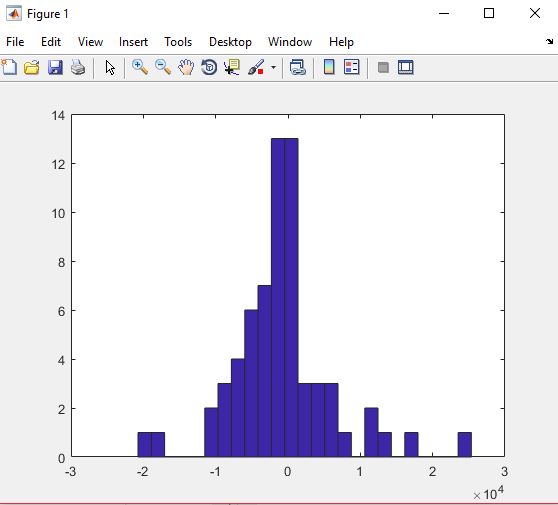
\includegraphics[width=2in,height=2in]{hist.PNG}
\caption{Simulación Histórica} 
\label{Figure 1} 
\end{center}
\end{minipage}
\end{figure}

En la Figura 1, se aprecia un histograma de frecuencia para los valores de los portafolios de inversión en orden ascendente. Parece tener una distribución, con una media cercana a 0. El VaR calculado fue de 19,233, indicando que, con un nivel de significancia del 90 por ciento, la máxima pérdida sería de 19233 pesos.

\ \\%

\section{Simulación MonteCarlo}

La simulación MonteCarlo, es un modelo paramétrico que utiliza la ecuación de rendimientos, utilizando como parámetros la desviación estándar (volatilidad), la media (valor esperado del activo) y DeltaW (la parte estocástica del modelo que contiene tato las correlaciones de los activos (eta), como la variable aleatoria con distribución normal (z)).

$$ R_{f}= \mu\Delta t + \sigma\Delta W  = \mu\Delta t + \sigma \: \sqrt{\Delta t} \: \epsilon = \mu\Delta t + \sigma  \: \sqrt{\Delta t} \: z \: \eta \: \: \: \: \: \: \: \: \: donde \: \epsilon = z \: \eta$$

El método consiste en la simulación repetida del cálculo de los rendimientos para la creación de portafolios, y poder estimar de esta forma el VaR correspondiente a una fecha en particular.

\ \\%
Para el cálculo del VaR por el método de simulación MonteCarlo, se calcularon los rendimientos de los activos y de estos se obtuvieron los valores promedio de sus rendimientos, la desviación estándar de los rendimientos, como la matriz de correlaciones. Con la matriz de correlaciones, se obtuvo una matriz "eta" que es el Cholesky de la matriz de correlaciones, la cual introduce en el modelo esa relación entre los activos. 

\ \\%
Se creó una matriz "z" que contiene valores aleatorios con distribución normal. Utilizando los valores iniciales de los activos, se simuló 1000 veces el valor del portafolio de inversión con montos de 100 mil, 100 mil y 300 mil pesos, para BIMBO, HOMEX e ICA respectivamente; siguiendo la ecuación anterior. Se guardaron los valores resultantes para cada portafolio para su análisis.

\ \\%
El VaR se calculó multiplicando el valor del primer decil de los valores de los portafolios para cada simulación ordenados de menor a mayor por la raíz cuadrada del incremento del tiempo a buscar respecto del último dato histórico.

\begin{figure}[h]
\begin{minipage}{7in}
\begin{center}
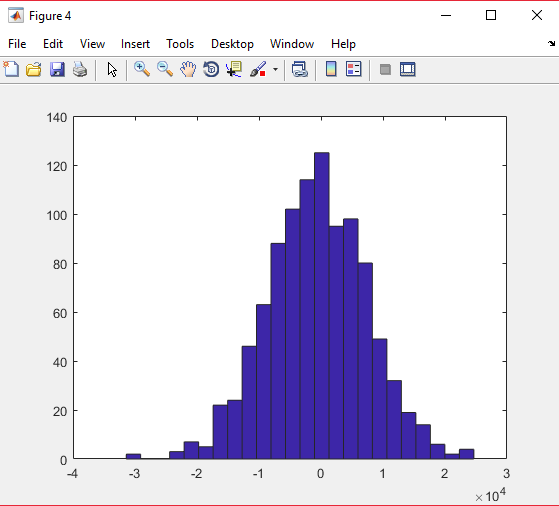
\includegraphics[width=2in,height=2in]{montecarlo.PNG}
\caption{Simulación MonteCarlo} 
\label{Figure 2} 
\end{center}
\end{minipage}
\end{figure}

En la Figura 2, se aprecia un histograma de frecuencia para los valores de los portafolios de inversión en orden ascendente. Parece tener una distribución, con una media cercana a cero. El VaR calculado fue aproximadamente 30 mil, indicando que, con un nivel de significancia del 90 por ciento para el 2 de octubre de 2017, la máxima pérdida sería de 30 mil pesos.

\section{Delta Normal}
Para el método Delta Normal, se debe considerar que los rendimientos de los activos que forman el portafolio, tienen una distribución normal. Del tal forma que la media y la desviación estándar del portafolio se definan por medio de:

$$E[R_{p}] = \omega ' E[R] \: \: \: \: \: \: \: \: \: \: \:\: \: \omega_{p}^2 = \omega ' (matriz\:de\:varianzas) * \omega$$ \: \: \: \: 

Donde $ \omega\:$ es la matriz de montos a invertir. Una vez calculado el valor promedio y la desviación estándar (raíz cuadrada de la varianza del portafolio), el VaR se calcula:
$$ VaR_{p} = (E_{p}-(\alpha \:\sigma_{p}))\:\sqrt{\Delta t}$$

Se calcularon las matrices, y se hicieron las multiplicaciones de matrices para obtener como resultado la media, varianza, y desviación estándar de los valores de los portafolios y se obtuvo como resultado la siguiente gráfica.

\begin{figure}[h]
\begin{minipage}{7in}
\begin{center}
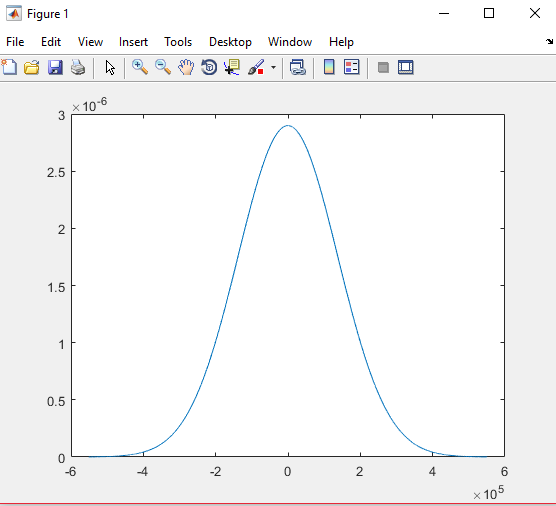
\includegraphics[width=2in,height=2in]{delta.PNG}
\caption{Delta Normal} 
\label{Figure 3} 
\end{center}
\end{minipage}
\end{figure}

En la Figura 2, se aprecia una función de densidad que representa los valores de los portafolios de inversión de acuerdo con el método Delta Normal. Parece tener una distribución, con una media cercana a cero. El VaR estimado para el portafolio conformado por montos de 100 mil, 100 mil y 300 mil pesos, para BIMBO, HOMEX e ICA respectivamente mediante el método de Delta Normal, es de 394,574, indicando que el valor máximo de pérdida esperado para el día 2 de octubre de 2017 es de 394,574 pesos, con un nivel de significancia del 90 por ciento.

\section{Conclusión}

\begin{table}[htb]
\centering
\begin{tabular}{|l|l|l|l|}
\hline
& \multicolumn{3}{c|}{VaR} \\
\cline{2-4}
& Simulación Histórica & MonteCarlo & Delta Normal\\
\hline \hline
\multirow{VaR a una semana} & 19,233 & 30,000 & 394,574\\ 
\cline{1-4}
Valor real ocurrido(Ganancia)& 6,115 & 6,115 & 6,115\\ 
\cline{1-4}
\end{tabular}
\caption{Tabla Comparativa VaR y Valor Real.}
\label{tabla:final}
\end{table}

Observando el Cuadro 1, se puede concluir que los VaR de los métodos de Simulación Histórica y MonteCarlo son muy similares. Sin embargo, el VaR obtenido mediante el método Delta Normal es significativamente más grande que el de los otros 2 métodos. Esto se puede deber a que os rendimientos de los activos, durante el periodo de tiempo elegido no tienen una distribución normal, siendo que en repetidas ocasiones el valor de los activos se mantuvieron constantes en sus valores de cierre.

\ \\%
En comparación con lo que sucedió realmente el día 2 de octubre de 2017, se puede decir que se cumplieron las predicciones. El día 2 de octubre, no hubo perdida, al contrario, hubo una ganancia de 6,115 pesos. Se cumple la predicción ya que el valor real no supero en pérdida ninguno de los 3 VaR que se calcularon.
\end{document}
